\documentclass[12pt]{article}
\usepackage[utf8]{inputenc}
\usepackage{float}
\usepackage{amsmath}
\usepackage{graphicx}

\usepackage[hmargin=3cm,vmargin=6.0cm]{geometry}
\topmargin=-2cm
\addtolength{\textheight}{6.5cm}
\addtolength{\textwidth}{2.0cm}
\setlength{\oddsidemargin}{0.0cm}
\setlength{\evensidemargin}{0.0cm}
\usepackage{indentfirst}
\usepackage{amsfonts}

\begin{document}

\section*{Student Information}

Name : Emre Geçit

ID : 2521581

\section*{Question 1}
Design a Turing machine which recognizes the language $L = {0^N1^N | N \geq 1}$.

$\Sigma = \{0, 1, \sqcup\}$, means that you cannot write any other symbol than these symbols.
\paragraph{Solution:\\}
Descriptions for the states:
\begin{itemize}
    \item State 0 (Initial state): If the tape head is on a 0, changes it with a blank space, moves the tape head to right, and passes to the state 1. If it is on a blank space, passes to the acceptance state.
    \item State 1: This state's task is finding the right end of the string. After finding the rightmost character in the string, the machine passes to state 2.
    \item State 2: If the tape head is on a 1, changes it with a blank space, moves the tape head to left, and passes to the state 3. If it is on a blank space, passes to the acceptance state.
    \item State 3: This state's task is finding the left end of the string. After finding the leftmost character in the string, the machine passes to state 0.
\end{itemize}
Note that in these descriptions, undefined transititons leads to rejection of the string.
\begin{figure}[bp!]
    \caption{Turing machine which recognizes the language $L = {0^N1^N | N \geq 1}$}
    \centering
    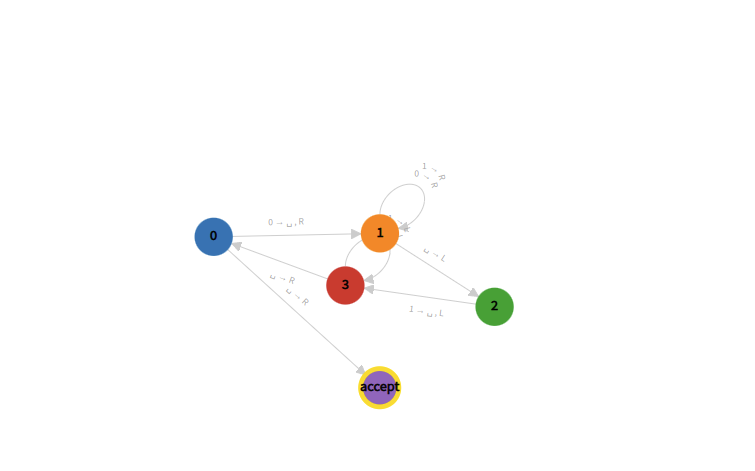
\includegraphics[width=12cm]{Q1/turingmachine.io_.png}    
\end{figure}

\newpage
\paragraph{Sample inputs:\\}
\begin{figure}[bp!]
    \caption{Input = 000111}
    \centering
    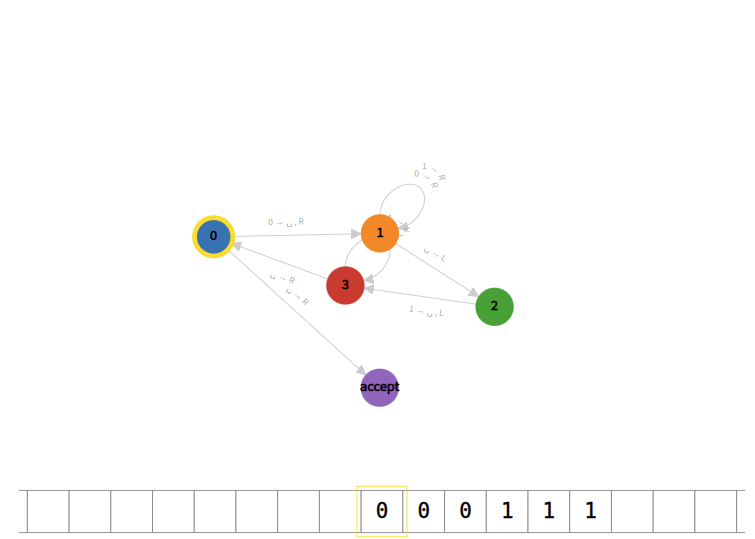
\includegraphics[width=12cm]{Q1/000111.png}    
\end{figure}
\begin{figure}[bp!]
    \caption{Input = 000111, Output = Accepted}
    \centering
    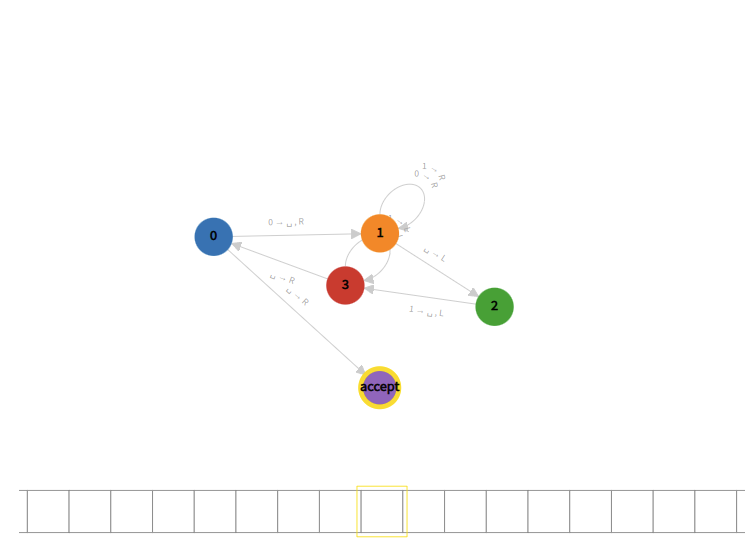
\includegraphics[width=12cm]{Q1/000111o.png}    
\end{figure}
\begin{figure}[bp!]
    \caption{Input = 0000111}
    \centering
    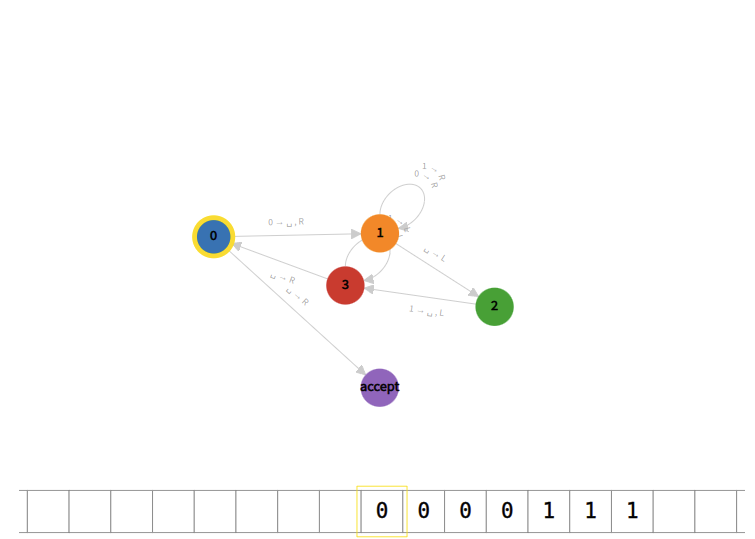
\includegraphics[width=12cm]{Q1/0000111.png}    
\end{figure}
\begin{figure}[bp!]
    \caption{Input = 0000111, Output = Rejected}
    \centering
    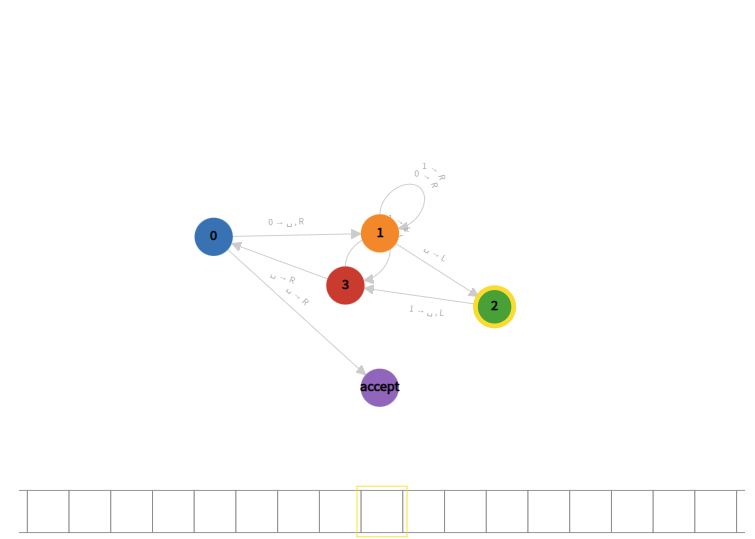
\includegraphics[width=12cm]{Q1/0000111o.png}    
\end{figure}
\begin{figure}[bp!]
    \caption{Input = 000011111}
    \centering
    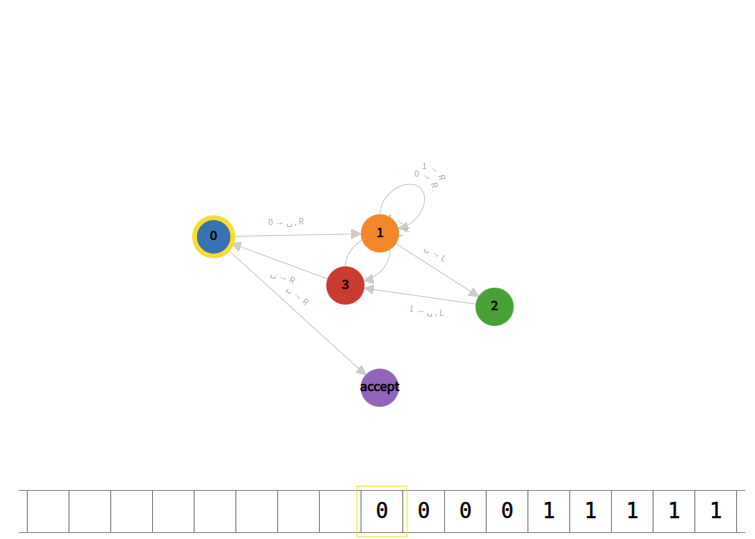
\includegraphics[width=12cm]{Q1/000011111.png}  
\end{figure}
\begin{figure}[bp!]
    \caption{Input = 000011111, Output = Rejected}
    \centering
    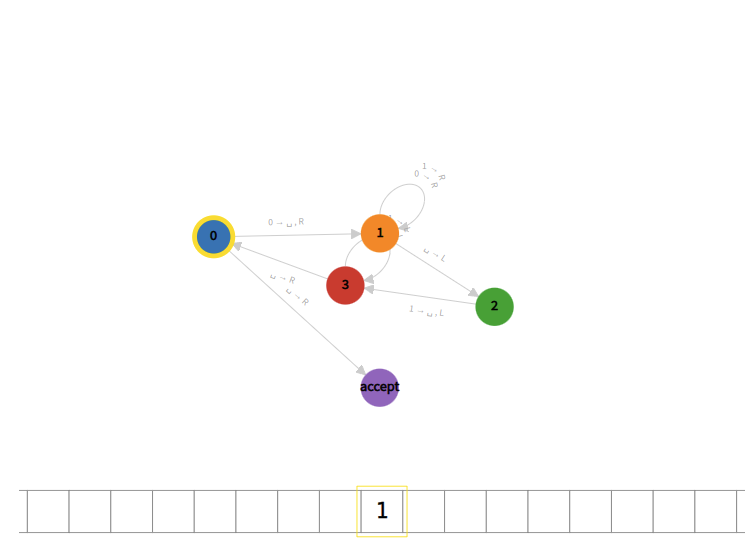
\includegraphics[width=12cm]{Q1/000011111o.png}  
\end{figure}
\begin{figure}[bp!]
    \caption{Input = 0001110}
    \centering
    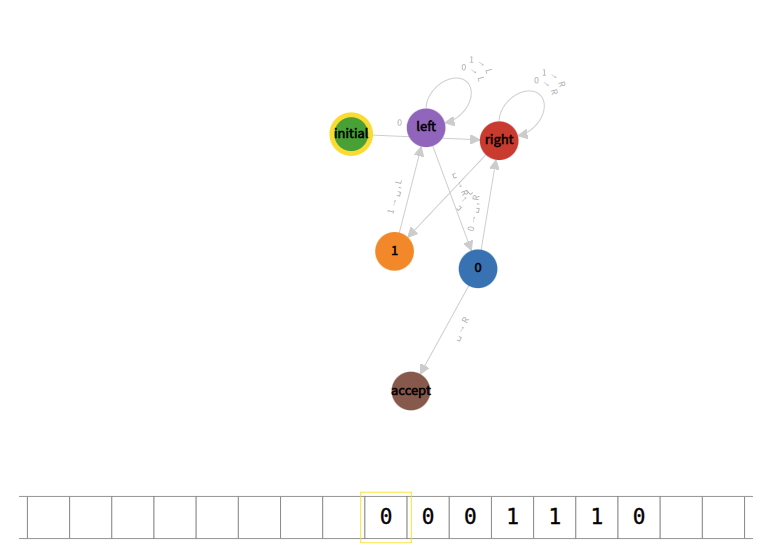
\includegraphics[width=12cm]{Q1/0001110.png}  
\end{figure}12cm
\begin{figure}[bp!]
    \caption{Input = 0001110, Output = Rejected}
    \centering
    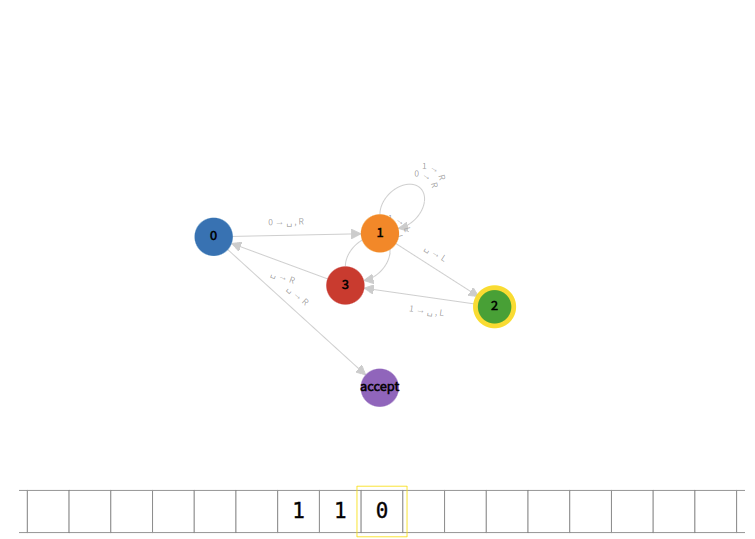
\includegraphics[width=12cm]{Q1/001101o.png}  
\end{figure}
\begin{figure}[bp!]
    \caption{Input = 100011}
    \centering
    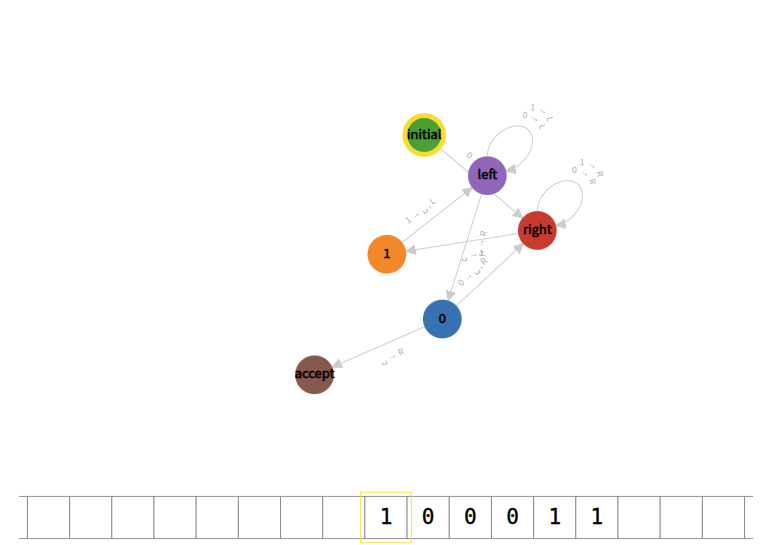
\includegraphics[width=12cm]{Q1/100011.png}
\end{figure}
\begin{figure}[bp!]
    \caption{Input = 100011, Output = Rejected}
    \centering
    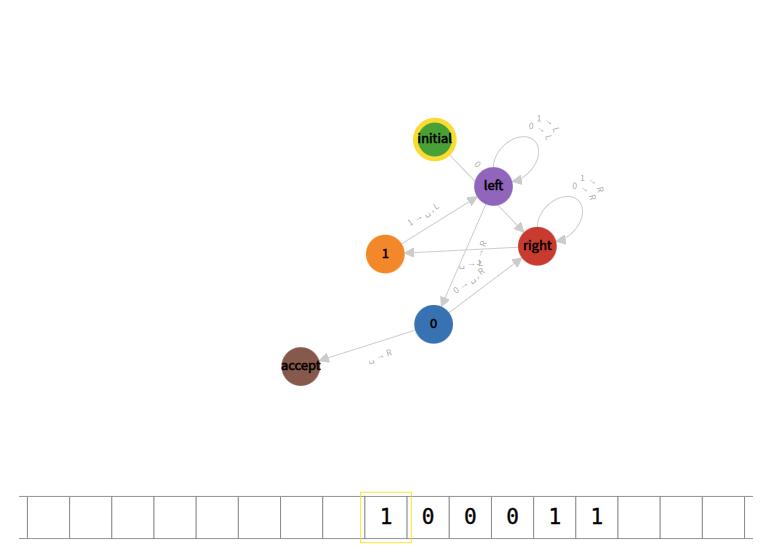
\includegraphics[width=12cm]{Q1/100011o.png}
\end{figure}
\newpage
\newpage
\newpage
\section*{Question 2}
\paragraph{a)}
\paragraph{b)}

\section*{Question 3}
\paragraph{a)}
\paragraph{b)}

\end{document}

